\documentclass[10pt,utf8,presentation,notheorems,xcolor=dvipsnames,compress]{beamer}
\usepackage{doclad}

%Тут можно вставить дополнительные пакеты

\title[Информационная система]{
Информационная система \newline «Better Row»
}

\author[Абдулов И.А.]{
  Абдулов Илья Александрович
}



\date{27 октября  2022}

\begin{document}

\begin{frame}
\titlepage
\end{frame}

\section<presentation>*{Содержание}

\begin{frame}
\frametitle{Содержание}
\tableofcontents
\end{frame}

\section{Введение}
\begin{frame}
\frametitle{Введение}
\begin{block}{Better Row}
Мобильное приложение, куда пользователь заносит данные своих тренировок, чтобы приложение показывало и сохраняло текущие показатели и прогресс. Использование приложения придаст тренировкам осознанности, что поможет в достижении лучшего результата.
\end{block}
\begin{block}{Цель практической работы 4}
Целью данной работы является описание предметной области функционирования и основной идеи будущего мобильного приложения.
\end{block}
\end{frame}

\section{Описание Better Row}

\subsection{Назначение и пользователи Better Row}
\begin{frame}
\frametitle{Назначение и пользователи Better Row}

\begin{block}{Назначение приложения}
Позволить пользователю сохранять данные о своих тренировках на концепте, чтобы в дальнейшем иметь возможность видеть свой прогресс.
\end{block}

\begin{block}{Основные пользователи}
Основными пользователями системы будут являться любители академической гребли и участники студенческой гребной лиги России.
\end{block}
\end{frame}

\section{Описание Better Row}

\subsection{Планируемый набор функций и прототип интерфейса}
\begin{frame}
\frametitle{Главное меню приложения}
Планируется реализовать три вкладки в главном меню: результаты и статистика, расписание тренировок, настройки приложения.
\begin{center}
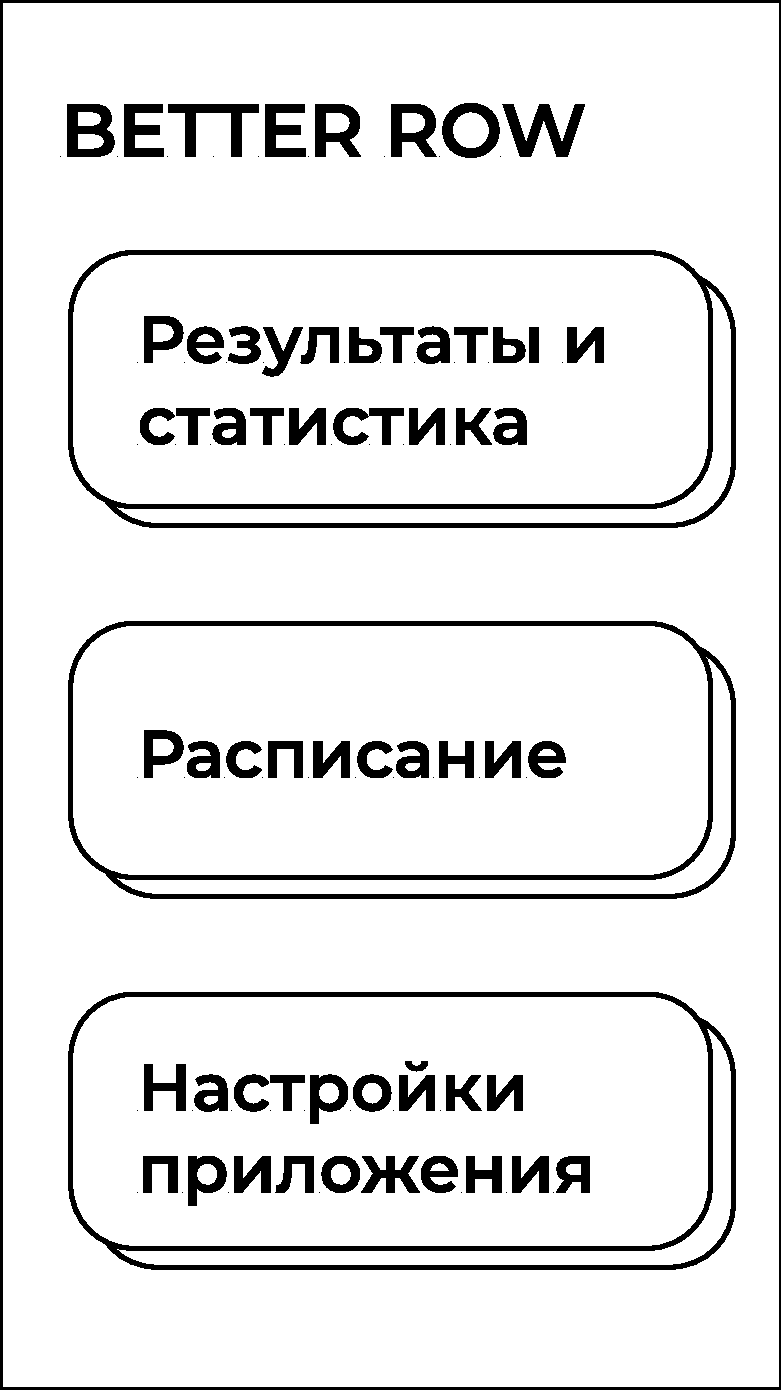
\includegraphics[scale=0.26]{iPhone 8 - 3.pdf}%
\end{center}
\end{frame}

\begin{frame}
\frametitle{Pезультаты и статистика}
Перемещение для просмотра тренировок по дням. При добавлении тренировки пользователь вводит дистанцию, время, темп заплыва на концепте и пульс.
\begin{center}
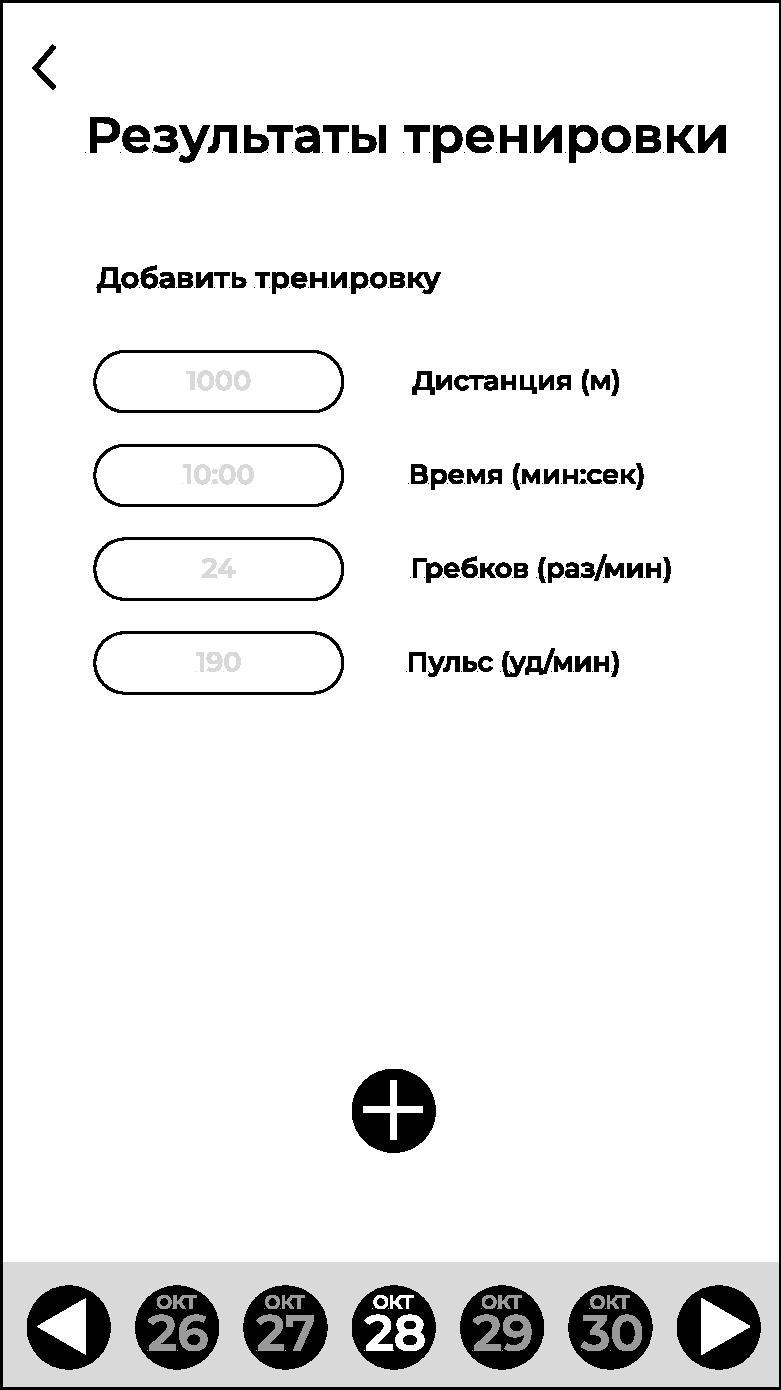
\includegraphics[scale=0.26]{iPhone 8 - 2}%
\end{center}
\end{frame}

\begin{frame}
\frametitle{Pезультаты и статистика}
При просмотре тренировок выводится средняя скорость заплыва и сравнение результатов с прошлыми тренировками.
\begin{center}
\includegraphics[scale=0.26]{iPhone 8 - 1}%
\end{center}
\end{frame}

\begin{frame}
\frametitle{Расписание тренировок}
Пользователь может всегда изменить расписание
\begin{center}
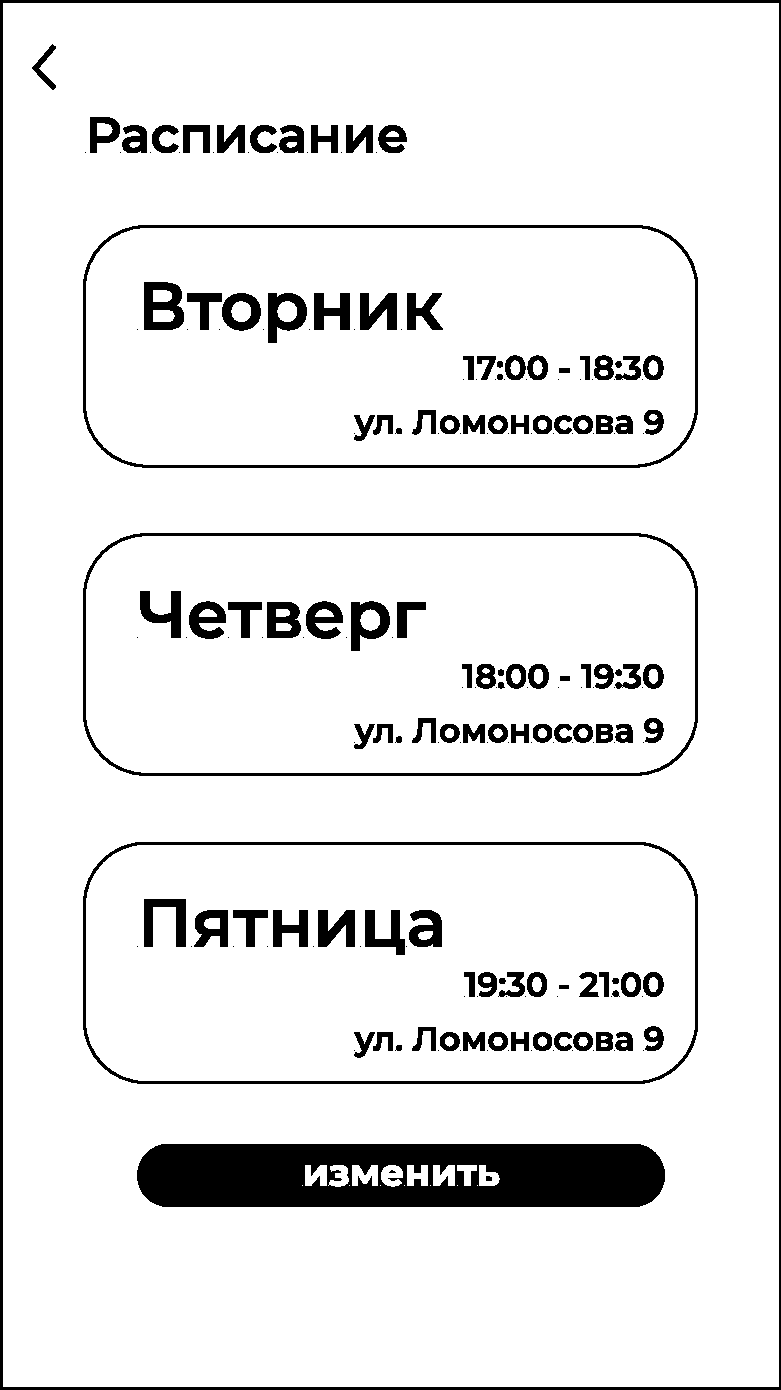
\includegraphics[scale=0.26]{iPhone 8 - 4}%
\end{center}
\end{frame}


\section{Аналоги}
\begin{frame}
\frametitle{Watersports Tracker}
Приложение, которое предоставляет статистику о тренировке на воде, отслеживая геолокацию смартфона.
\begin{center}
\includegraphics[scale=0.3]{Watersports Tracker}%
\end{center}
\end{frame}

\begin{frame}
\frametitle{RowingCoach 4.0}
Приложение предоставляет статистику и все показатели тренировки, отслеживая местоположение пользователя.
\begin{center}
\includegraphics[scale=0.3]{RowingCoach}%
\end{center}
\end{frame}

\section{Заключение}
\begin{frame}
\frametitle{Заключение}
\begin{block}{В практической работе}
\begin{itemize}
 \item Представлено мобильное приложение «Better Row»
 \item Описана предметная область функционирования приложения и основная идея приложения
 \item Представлен прототип интерфейса приложения
\end{itemize}
\end{block}
\end{frame}
\end{document}
